\documentclass[aspectratio=169]{beamer}
\usepackage[english, russian]{babel}
\usepackage[utf8]{inputenc}
 \usepackage{pgf}

\begin{document}

\begin{frame}
\Large
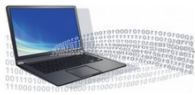
\includegraphics[width=2cm]{logo} {\bf Офисное программное обеспéчение}
\begin{flushleft}
\footnotesize
К офисному программному обеспечению (ПО) относят наиболее часто
применяемые в офисной работе программы для редактирования электронных документов.
Существует более 30 серьёзных офисных пакетов разных производителей. Они различаются по
составу и функционалу, но почти во всех присутствуют следующие три обязательных компонента:
\begin{itemize}
\itemТекстовый процессор (текстовый редактор) – ТП.
\itemЭлектронная таблица (табличный процессор) – ЭТ.
\itemПрограмма подготовки презентаций – ПП.
\end{itemize}
{\bf Форматы файлов офисного ПО (наиболее популярные)}
\begin{itemize}
\itemТП: doc, docx, odt
\itemЭТ: xls, xlsx, ods
\itemПП: ppt, pptx, odp
\end{itemize}
{\bf Интересные факты}
\begin{itemize}
\itemФорматы doc/xls/ppt до сих пор «закрыты» (по состоянию на 2017 год), хотя в разное время
компания Microsoft предоставляла временный и/или частичный доступ к ним.
\itemФорматы docx, odt, xlsx, ods, pptx, odp – это zip-архивы с xml- и медиафайлами.
\itemПП:Криптографическая защита в doc, xls, ppt крайне слабая (даже для длинных паролей).
\end{itemize}
\end{flushleft}
\end{frame}
\begin{frame}
\Large
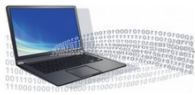
\includegraphics[width=2cm]{logo} {\bf Программное обеспéчение или обеспечéние}

\normalsize
{\bf  Обеспечéние}
\tiny
\begin{enumerate}
\itemОрфоэпический словарь (Аванесов, 1988):
обесп чение, ! не рек. обеспеч ние. ѐ ѐ
\itemРусское словесное ударение (Зарва, 2002): обесп чение [не обеспеч ние] ѐ ѐ
\itemСловарь трудностей произношения и ударения в современном русском языке (Горбачевич, 2002):
обесп чение (не рекомендуется обеспеч ние) ѐ ѐ
\itemУчебный словарь трудностей произношения и ударения в современном русском языке (2004,
Гостеева): Обесп чение. Не рек. обеспеч ние ѐ ѐ
\itemСовременный толковый словарь русского языка (Ефремова, 2000): обесп чение; обеспеч ние разг. ѐ ѐ
\itemДавайте говорить правильно (Вербицкая, 2008): обесп чение, в проф. речи обеспеч ние
\end{enumerate}
\normalsize
{\bf  Обеспéчение}
\tiny
\begin{enumerate}
\itemБольшой толковый словарь (Кузнецов, 2009).
\itemТолковый словарь (Ожегов, 1992).
\itemТолковый словарь (Ушаков, 1940).
\itemМорфемно-орфографический словарь (Тихонов, 2002).
\item Collins Russian Dictionary (2000).
\itemОнлайн-словарь http://www.wiktionary.org
\itemОнлайн-словарь http://en.bab.la
\itemОнлайн-словарь http://ru.forvo.com
\end{enumerate}
\normalsize
{\bf  Обеспéчение и обеспечéние}
\tiny
\begin{enumerate}
\itemРусский орфографический словарь (Лопатин, 2004).
\itemТолковый словарь (Дмитриев, 2003).
\end{enumerate}
\end{frame}
\begin{frame}
\Large
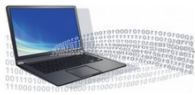
\includegraphics[width=2cm]{logo} {\bf Наиболее популярные офисные пакеты}
\normalsize
Данные о популярности офисных пакетов получены с помощью анализа статистики,
собранной с помощью сайта trends.google.com. В таблице пакеты приведены по
убыванию популярности. Стоимость указана для desktop-версий.
\begin{center}
\scriptsize
\begin{tabular}{| c | c | c | c |}
\hline
Название & Особенности & Cтоимость, руб. & Исходный код\\ \hline
Google Docs & Узкая ориентация на публичные облачные решения & бесплатно & закрытый\\ \hline
Microsoft Office & Имеет наиболее богатый функционал & 5000–35000 & закрытый\\ \hline
LibreOffice & Слабая поддержка одновременного редактирования & бесплатно & открытый\\ \hline
iWork & Узкая ориентация на технику фирмы Apple & бесплатно & закрытый\\ \hline
WordPerfect Office & Ориентация на рынок ПК & 5000–25000 & закрытый\\ \hline
OnlyOffice & Ориентация на облачные решения & бесплатно & открытый\\ \hline
\end{tabular}
\end{center}
\end{frame}
\begin{frame}
\Large
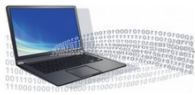
\includegraphics[width=2cm]{logo} {\bf Формат ODF и ГОСТ России}
\footnotesize

Открытый бесплатный формат ODF (Open Document Format) позволяет обеспечить
возможность долгосрочного хранения электронных документов без привязки к «капризам»
конкретного производителя офисного ПО. Стандарты ODF описывают 16 форматов файлов
(документы, картинки, таблицы, формулы, диаграммы), включая odt, ods, odp.
{\bf Стандратизация ODF в России (во многих других странах ситуация похожая)}
\begin{itemize}
\item ODF 1.0 был описан и введён в действия по ГОСТ 26300-2010 (с 1 июня 2011 г.)
\item ГОСТ 26300-2010 должен использоваться для документооборота в госструктурах.
\item Стандартизация ODF не означает навязывание LibreOffice/OpenOffice.
\end{itemize}
{\bf Проблемы ГОСТ 26300-2010}
\begin{itemize}
\itemТекущая версия ODF уже 1.2 (в ней исправлены многие проблемы версии 1.0)
\itemНе описаны спецификации скриптов и макросов.
\itemНе описано применение цифровых подписей.
\itemНе описан язык описания формул.
\itemНе допускается использование таблиц в презентациях.
\end{itemize}
\end{frame}
\begin{frame}
\Large
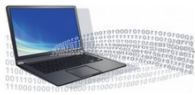
\includegraphics[width=2cm]{logo} {\bf «Продвинутые» функции текстовых процессоров и электронных таблиц}
\footnotesize

В школе офисные пакеты изучаются очень подробно. Однако есть ряд немаловажных
функций текстовых процессоров и электронных таблиц, о которых в школе почти не говорят.
{\bf Текстовый процессор}
\begin{itemize}
\itemКонцепция стилей для оформления текстового документа
\itemАвтонумерация рисунков, таблиц, формул
\itemМакросы для автоматизации повторяющихся действий
\itemАвтозаполнение «мусорным» текстом
\end{itemize}
{\bf Табличный процессор}
\begin{itemize}
\itemРасчёт доверительного интервала
\itemФильтры содержимого таблиц
\itemЗапрет на ввод некорректных значений в ячейку.
\itemУсловное форматирование
\itemИнструмент «Подбор параметра»
\end{itemize}
Рассматриваемые далее примеры выполнены в LibreOffice 5.1, однако в других офисных
пакетах есть аналогичные функции (даже их названия почти всегда дословно совпадают).
\end{frame}
\end{document}